%\chapter{CountMax:数据平面的流量测量工具}
% \chapter{SDN中流量测量sketch的研究现状}

本章将介绍4种典型的用于流量测量的sketch,并分析它们为何无法适用于SDN。

\section{Count-Min\cite{cormode2004improved}}

\begin{figure}[h]
	\centering
	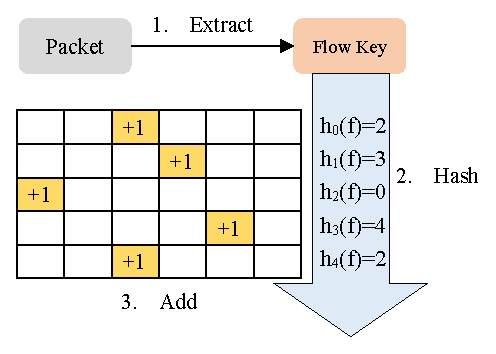
\includegraphics[width=0.8\linewidth]{fig/countmin2.eps}
	\caption{Count-Min的更新过程}\label{fig:countmin}
\end{figure}

如图\ref{fig:countmin}所示,Count-Min sketch的存储形式是一个高度为$d$、长度为$w$的二维数组(也称为\textit{bitmap})。数组中的每个位置称为一个“格子”(slot),格子中包含了一个从0开始的计数器。
数组中的每一行都拥有一个哈希函数,可以将任意流ID,如5元组,映射到$\{0,1,...,w-1\}$之间的某个数。

当一个数据包到达时,Count-Min首先读取它的流ID,然后对于数组的每一行,使用它的哈希函数将ID映射为一个数,用这个数作为索引定位到相应的格子,将格子中的计数器增加。
在统计数据包数的情况下,将计数器加一;在统计数据流量的情况下则将计数器增加相当于数据包字节数的大小。

\chapter{CountMax:轻量级的流量测量sketch}\label{chap:countmax}
本章首先说明CountMax的设计目标,紧接着详细介绍CountMax的算法细节、性能分析以及CountMax的应用,随后通过仿真模拟和系统集成测试对CountMax和其它两种sketch的综合性能进行对比。


\section{算法设计}
首先我们确定CountMax算法设计的目标,然后再来介绍算法的具体设计。
CountMax的算法设计包含两部分,其一为统计信息的记录和更新,其二为统计信息的查询。

\subsection{设计目标}
根据第\ref{chap:sketch}章中对已有的sketch方案的分析,为了解决已有sketch的不足,CountMax的设计目标有以下几点:
\begin{enumerate}
	\item 大流识别。在实际应用中我们很难获得关于大流的先验知识,因此CountMax必须负责将大流的ID从成千上万的流当中识别出来。
	\item 更低的计算负载。CountMax应当占用尽可能少的CPU资源,一方面可以应对更重的网络负载,另一方面也为交换机上的其它应用留出了空间。
	\item 较低的测量误差。CountMax对大流流量的估算误差应当可控,且处于可接受的较低范围内。
	\item 追踪更多的大流。在消耗同样的存储空间的前提下,被CountMax所追踪的大流越多,就可以提供越多的有用信息,提升重路由等应用的质量。
\end{enumerate}

\subsection{设计简述}
为了尽量降低计算负载,CountMax摒弃了提高复杂度的辅助数据结构。我们选择仿照Count-Min的设计,只使用bitmap存储数据。
同时,为了识别大流,CountMax在bitmap的每一个格子中都增加了一个存放流ID的字段。
当发生哈希冲突时,Count-Min不对流做区分,全部累加到计数器当中。这样的做法导致了Count-Min无法记录大流的ID。
因此,在CountMax的设计中,在多条流发生哈希冲突时,会根据当前流的ID和bitmap中现有的流ID的关系来选择不同的操作。
可简要描述为:若二者相同,则计数器增加;若二者不同,则计数器减去相应的大小。若减去后的结果为负数,对应格子中的流ID字段也会更改为当前流的ID。
由于网络中的大流的大小往往是小流的上千倍,当一条大流和多个小流碰撞时,这样的算法可以在绝大多数情况下保证最终记录下来的流ID是大流的ID。
而对于大流之间的哈希碰撞,则可以通过增加bitmap行数的方式降低其概率。

\subsection{统计信息记录}
为了记录统计信息,我们维护一个有$d$行、$w$列的bitmap。
Bitmap中的每个格子包含两个字段:$Key$和$Counter$。参数$d$和$w$的意义将在后文讨论。
和bitmap一起的还有$d$个不同的哈希函数$\{h_{1},...,h_{d}\}$。
每个哈希函数$h_j$都能将任意流的ID(如五元组)单向映射为一个介于$0$和$w-1$之间的整数:
\begin{equation}
\notag h_j: \{...\} \to \{0, ..., w-1\}
\end{equation}

\begin{algorithm}[htb]
    \small
    \SetAlgoLined
    \KwData{$f_i$:流的ID; $c_i$:数据包的大小}
  
    \For{$j$从0到$d-1$}{
        $u_j = h_{j}(f_i)$\;
        $f' = Key_{j}[u_j]$\;
        \eIf{$f_i == f'$}{
            $Counter_{j}[u_j] = Counter_{j}[u_j]+c_i$\;
        }{
            \If{$Counter_{j}[u_j] > c_i$}{
                $Counter_{j}[u_j] = Counter_{j}[u_j]-c_i$\;
            }{
                $Counter_{j}[u_j] = c_i-Counter_{j}[u_j]$\;
                $Key_{j}[u_j] = f$\;
            }
        }
    }
    \caption{CountMax对每个数据包的处理过程}
    \label{alg:count_max}
\end{algorithm}
当交换机接收到第$i$号数据包时,首先从数据包中解析出流的ID,记为$f_i$。对于bitmap中的第$j$行,先计算$f_i$的哈希值$u_{j}=h_{j}(f_i)$作为索引。
如果$Key_{j}[u_{j}]$与$f_i$相同,那么对应的$Counter_{j}[u_{j}]$就会加上数据包的大小,记做$c_i$。否则比较$Counter_{j}[u_{j}]$和$c_i$之间的大小。
如果$Counter_{j}[u_{j}]$\textbf{大于}$c_i$,那么$Counter_{j}[u_{j}]$就减去$c_i$。写成表达式即为$Counter_{j}[u_{j}] = Counter_{j}[u_{j}] - c_i$。
如果$Counter_{j}[u_{j}]$\textbf{小于}$c_i$,则令$Counter_{j}[u_{j}]=c_i - Counter_{j}[u_{j}]$,并且将$Key_{j}[u_{j}]$替换为$f_i$。

对bitmap中的每一行迭代上述过程。算法\ref{alg:count_max}详细描述了这一算法。

\subsection{流量信息查询}
%\input{query.tex}
要查询流$f_i$的统计信息,首先从每一行中分别查询。对于sketch中的第$j$行,采用如下的方法获取$f_i$在当前行内的估计$\hat{a}_{i_{j}}$:
\begin{equation}
\hat{a}_{i_{j}}=\left\{
\begin{aligned}
Counter_{j}[h_j(f_i)]&\text{, 若 $f_i=Key_{j}[h_j(f_i)]$}\\
0&\text{, 若 $f_i \ne Key_{j}[h_j(f_i)]$}
\end{aligned}
\right.
\end{equation}

要推断流的流量大小,我们用上述方法查询每一行,从得到的结果中选取最大值作为估计值。
\begin{equation}
\label{eq:query}
\hat{a}_{i}=\max{\{\hat{a}_{i_{j}} , \forall j\}}
\end{equation}

\section{算法分析}\label{sec:analysis}
\label{subsec:analysis}
%\input{analysis.tex}

CountMax具有找出大流的能力。在分析CountMax的具体性能之前,首先对“大流”进行定义。
在网络中,随着流量分布的变化,字面意义上的top-$k$,即网络中流量最大的$k$条流的特征很难量化。因此,我们采用“heavy hitter”作为大流的定义。

给定网络中的所有流的集合,其中总共有$n$条流,所有流的流量之和是$F$。给定一个参数$\delta$ ($0<\delta \le 1$),则每一条流量大于或等于$\delta\cdot F$的流就称为这个集合中的$\delta$-``heavy hitter"。

\subsection{近似性能分析}
本小节将证明,在一定概率内,CountMax可以对heavy hitter的估计值有着可控的近似比。

\begin{theorem}
	\label{tm:query}
    对每条$\delta$-heavy hitter流$f_i$,令$\hat{a}_i$和$a_i$分别表示$f_i$的估算流量和实际流量。
    令$\tilde{d}$表示bitmap中记录有$f_i$的行的数目(即满足$Key[h(f_i)] = f_i$的行数),$e$代表自然对数的底,如下不等式始终满足:
	\begin{equation}
	\label{eq:hhacc}
	Pr[1-\frac{e}{w\cdot \delta}\le \frac{\hat{a}_i}{a_i} \le 1] \ge 1-e^{-\tilde{d}}
	\end{equation}
\end{theorem}

\begin{proof}
首先,由CountMax的性质易知,$\hat{a}_i$始终不大于$a_i$,即:
\begin{equation}
    \hat{a}_i/{a_i} \le 1
\end{equation}

接下来引入变量$I_{i,k,j}$来指示$f_i$和$f_k$两条流是否在第$j$行发生哈希冲突。即:
\begin{equation}
    I_{i,k,j}=\left\{
    \begin{aligned}
    1&\text{, if ($f_i \ne f_k $ ) $\land $ ($h_j(f_i)=h_j(f_k)$)}\\
    0&\text{, otherwise}
    \end{aligned}
    \right.
\end{equation}
由于哈希函数在理论上是独立的,因此对$f_i$和$f_k$的哈希计算可视为两个独立实验。又因为对不同的输入,理想的哈希函数将其散列到每个格子的概率是均等的,因此有:
\begin{equation}
    E(I_{i,k,j})=Pr[h_j(f_i)=h_j(f_k)] = \frac{1}{w}
\end{equation}

接下来定义变量$X_{i,j}$,令其表示在第$j$行中和$f_i$产生了哈希冲突的所有流的流量之和。即:
\begin{equation}\label{eq:xij}
    X_{i,j}=\sum\nolimits_{k=1}^{n}I_{i,k,j}\cdot a_k
\end{equation}

由于当$Key[h_j(f_i)]\ne f_i$时,查询的结果是0,因此必须找到$Key[h_j(f_i)] = f_i$的充分条件。
对于第$j$行,如果 $a_i > X_{i,j}$,也就是$a_i$大于这个格子所处理的总流量的一半,根据鸽巢原理,无论数据包的到达顺序如何,$Key[h_j(f_i)]$ 都必然是 $f_i$,并且$Counter[h_j(i)]\ge a_i-X_{i,j}$。
也就是说,对于$f_i$而言,$\tilde{d}$大于等于满足$a_i > X_{i,j}$的行的数量。
另外,如果$a_i \le X_{i,j}$,因为$Counter[h_j(i)]$永远不会为负,因此$Counter[h_j(i)]\ge a_i-X_{i,j}$依旧成立。

\begin{equation}\label{eq:ai_xij}
    Counter[h_j(i)]\ge a_i-X_{i,j}
\end{equation}

根据等式\eqref{eq:xij}可得:
\begin{equation}\label{eq:ex}\notag
E(X_{i,j})=E(\sum_{k=1}^{n}I_{i,k,j}\cdot a_k)\le\sum_{k=1}^{n} a_k\cdot E(I_{i,k,j})\le \frac{1}{w}\sum_{k=1}^{n}a_k.
\end{equation}


再根据$\delta$的定义,若$f_i$是$\delta$-heavy hitter,则网络中的总流量不超过$\frac{a_i}{\delta}$。因此:
\begin{equation}\label{eq:ex-delta}
E(X_{i,j})\le \frac{1}{w}\sum_{k=1}^{n}a_k\le \frac{1}{w}\cdot \frac{a_i}{\delta}
\end{equation}

综合以上结论,可以进行如下的推导。为方便起见,“$\forall j$”在这里代表“ $\forall j\in \{j|Key[h_j(f_i)] = f_i\}$”。
\begin{align}\notag
&Pr[\hat{a}_i< a_i-\frac{e}{w}\cdot\frac{a_i}{\delta}]\\\notag
&=Pr[\forall j, Counter[h_j(f_i)]<a_i-\frac{e}{w}\cdot\frac{a_i}{\delta} ]\\\notag
&\le Pr[\forall j, a_i-X_{i,j} <a_i-\frac{e}{w}\cdot\frac{a_i}{\delta} ] \text{ (根据不等式\eqref{eq:ai_xij})}\\\notag
&=Pr[\forall j, X_{i,j} > \frac{e}{w}\cdot\frac{a_i}{\delta} ]\\\notag
&\le Pr[\forall j, X_{i,j}>e\cdot E(X_{i,j})]\text{\ \ (根据马尔可夫不等式)}\\\notag
&<e^{-\tilde{d}}
\end{align}
	
将该不等式左侧的条件取反,可得结论:
\begin{equation}
Pr[\frac{\hat{a}_i}{a_i} \ge 1-\frac{e}{w\cdot \delta}]\ge 1-e^{-\tilde{d}}
\end{equation}

定理\ref{tm:query}得证。
\end{proof}


接下来分析$\tilde{d}$的数学期望。

\begin{theorem}\label{tm:acc}
对任何$\delta$-heavy hitter,$E[\tilde{d}]\ge d\cdot(1-1/(w\cdot\delta))$。
\end{theorem}

\begin{proof}
对于$\delta$-heavy hitter流 $f_i$以及bitmap中的第$j$行,根据上一节的推断,如果$a_i > X_{i,j}$那么$Key[h(f_i)] $ 一定为 $f_i$。

根据马卡洛夫不等式和不等式\eqref{eq:ex-delta},可得:
\begin{align}\notag
	Pr[X_{i,j}>a_i] &\le \frac{E[X_{i,j}]}{a_i}\\\notag
	&\le \frac{1}{w}\cdot\frac{a_i}{\delta}\cdot\frac{1}{a_i}\\
	&\le \frac{1}{w\cdot\delta}
\end{align}
因此 $Pr[Key[h_j(f_i)]=f_i]\ge 1- Pr[X_{i,j}>a_i] \ge 1-\frac{1}{w\cdot\delta}$。
    
由于bitmap中的每一行是独立的,因此$E[\tilde{d}]\ge d\cdot(1-1/(w\cdot\delta))$。
\end{proof}

\subsection{时间复杂度分析}
\begin{theorem}\label{tm:time}
CountMax对一个数据包进行处理的过程的时间复杂度是$O(d)$。
\end{theorem}

\begin{proof}
由于每一行的操作是固定的一次哈希、一次比较、一次加法,因而每行的时间复杂度是$O(1)$。
CountMax总共有$d$行,所以时间复杂度是$O(d)$。
\end{proof}




\section{CountMax在SDN中的应用}
本节介绍使用CountMax在SDN中进行重路由的应用,还提出了一种协作式的部署方式。
\subsection{借助CountMax进行重路由}\label{sec:flowrerouting}
流的重路由对于许多实际应用都是必要且十分重要的,如链路负载均衡以及链路中断时的重新寻路\cite{xu2017incremental}
。对于这些应用,网络中的大流的流量统计信息更加重要\cite{xu2017scalable}。

通过周期性地收集交换机的统计数据,控制器可以监控链路的流量负载。当控制器发现某条链路负载过重时,就需要对流进行重路由。
如果在交换机上安装了CountMax,控制器就可以收集CountMax中的信息,从而找出大流的集合,记为 $\Gamma^e$。
由于大流的流量占据了了网络整体流量中的大部分,因此通过采用各种算法对这些大流进行重路由,就可以快速有效地优化链路负载。
例如,我们可以利用一个简单的贪心法来重路由这些大流。首先将大流按照流量降序排列,然后按照顺序,控制器对每条流寻找一个占用率最低的路径作为新的路由。
在为所有大流都找好了新路径之后,将这些路径下发到交换机中\cite{jin2014dynamic} \cite{xu2017joint}。

这一过程中只对大流进行了重路由,而大流的数量和网络中流的总数相比非常少,因此重路由所需的时间也大幅减少。
由于CountMax的存储占用很小,因此收集CountMax的信息也不会为控制器带来明显的负载。


% \section{近似性能和计算负载的初步模拟}
% 小节\ref{sec:analysis}中的分析当中多次使用了不等式缩放、马尔可夫不等式,因此最终得到的结论颇为宽松。
% 为了更清楚的了解CountMax的实际性能,我们用C语言实现了CountMax并进行了一系列模拟。关于模拟环境的详细介绍请参见第XXXX章。
\begin{figure}[h]
	\centering
	\begin{minipage}[t]{0.48\linewidth}		
		%\begin{figure}[!t]
		\centering
		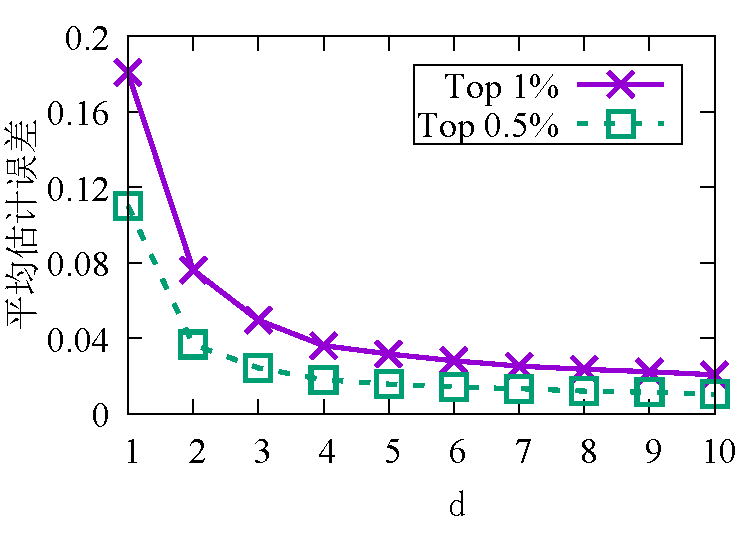
\includegraphics[width=\linewidth]{fig/cm_d_err.pdf}
		\caption{\textnormal{CountMax近似误差与$d$的关系}}
		\label{fig:cm,d,acc}
		%\end{figure}
	\end{minipage}\vspace{-0.6em}
\hspace{0.4em}
	\begin{minipage}[t]{0.48\linewidth}
        \centering
		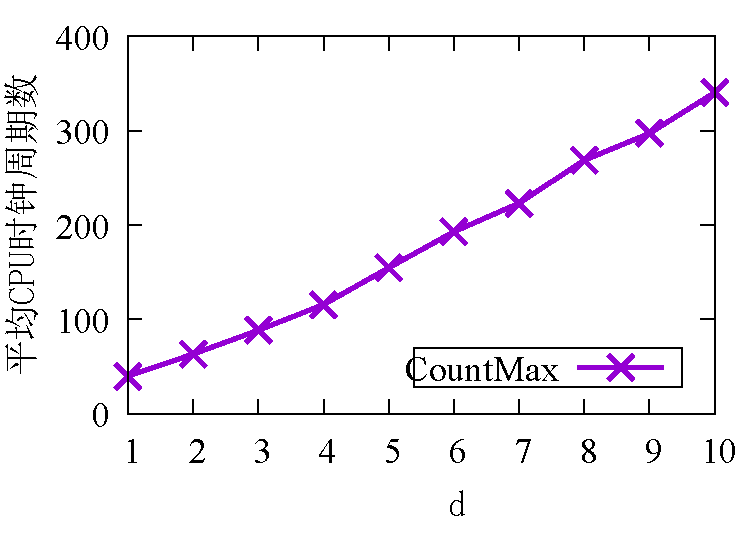
\includegraphics[width=\linewidth]{fig/cm_d_cpu.pdf}
		\caption{\textnormal{CountMax处理一个数据包的平均CPU周期数}}
		\label{fig:cm,d,cpu}
	\end{minipage}\vspace{-0.6em}
\hspace{0.1em}
\end{figure}

\subsection{CountMax的协作式部署}\label{sec:coop}
要进一步降低CountMax在交换机上的计算负载,主要有两种方法。
根据定理\ref{tm:time},CountMax处理单个数据包的时间复杂度是$O(d)$,因此第一种方法就是通过减少$d$的值来降低计算负载。

图\ref{fig:cm,d,acc}描述了CountMax在不同的行数下,对网络中前1\%或0.5\%的流的流量估计的误差。
关于测试环境的具体介绍请参见第\ref{sec:simulation}节。图\ref{fig:cm,d,acc}中的测试对应的是其中Spine-Leaf拓扑、20万条流、$k=2000$、非协作式的情况。
由图中我们可以看到,随着$d$的增长,估计误差一开始迅速降低,但随后降低的速度大幅放缓。$d=3$时的误差和$d=10$时的误差差别很小。
当$d=2$时,误差已经控制在10\%以内。

图\ref{fig:cm,d,cpu}描述了CountMax处理数据包所需的CPU时钟周期随$d$的变化而变化的情况。
图中的结果显示,CountMax的处理一个包的计算负载和$d$大致呈线性增长,同时印证了定理\ref{tm:time}。

\begin{figure}[h]
   \centering
   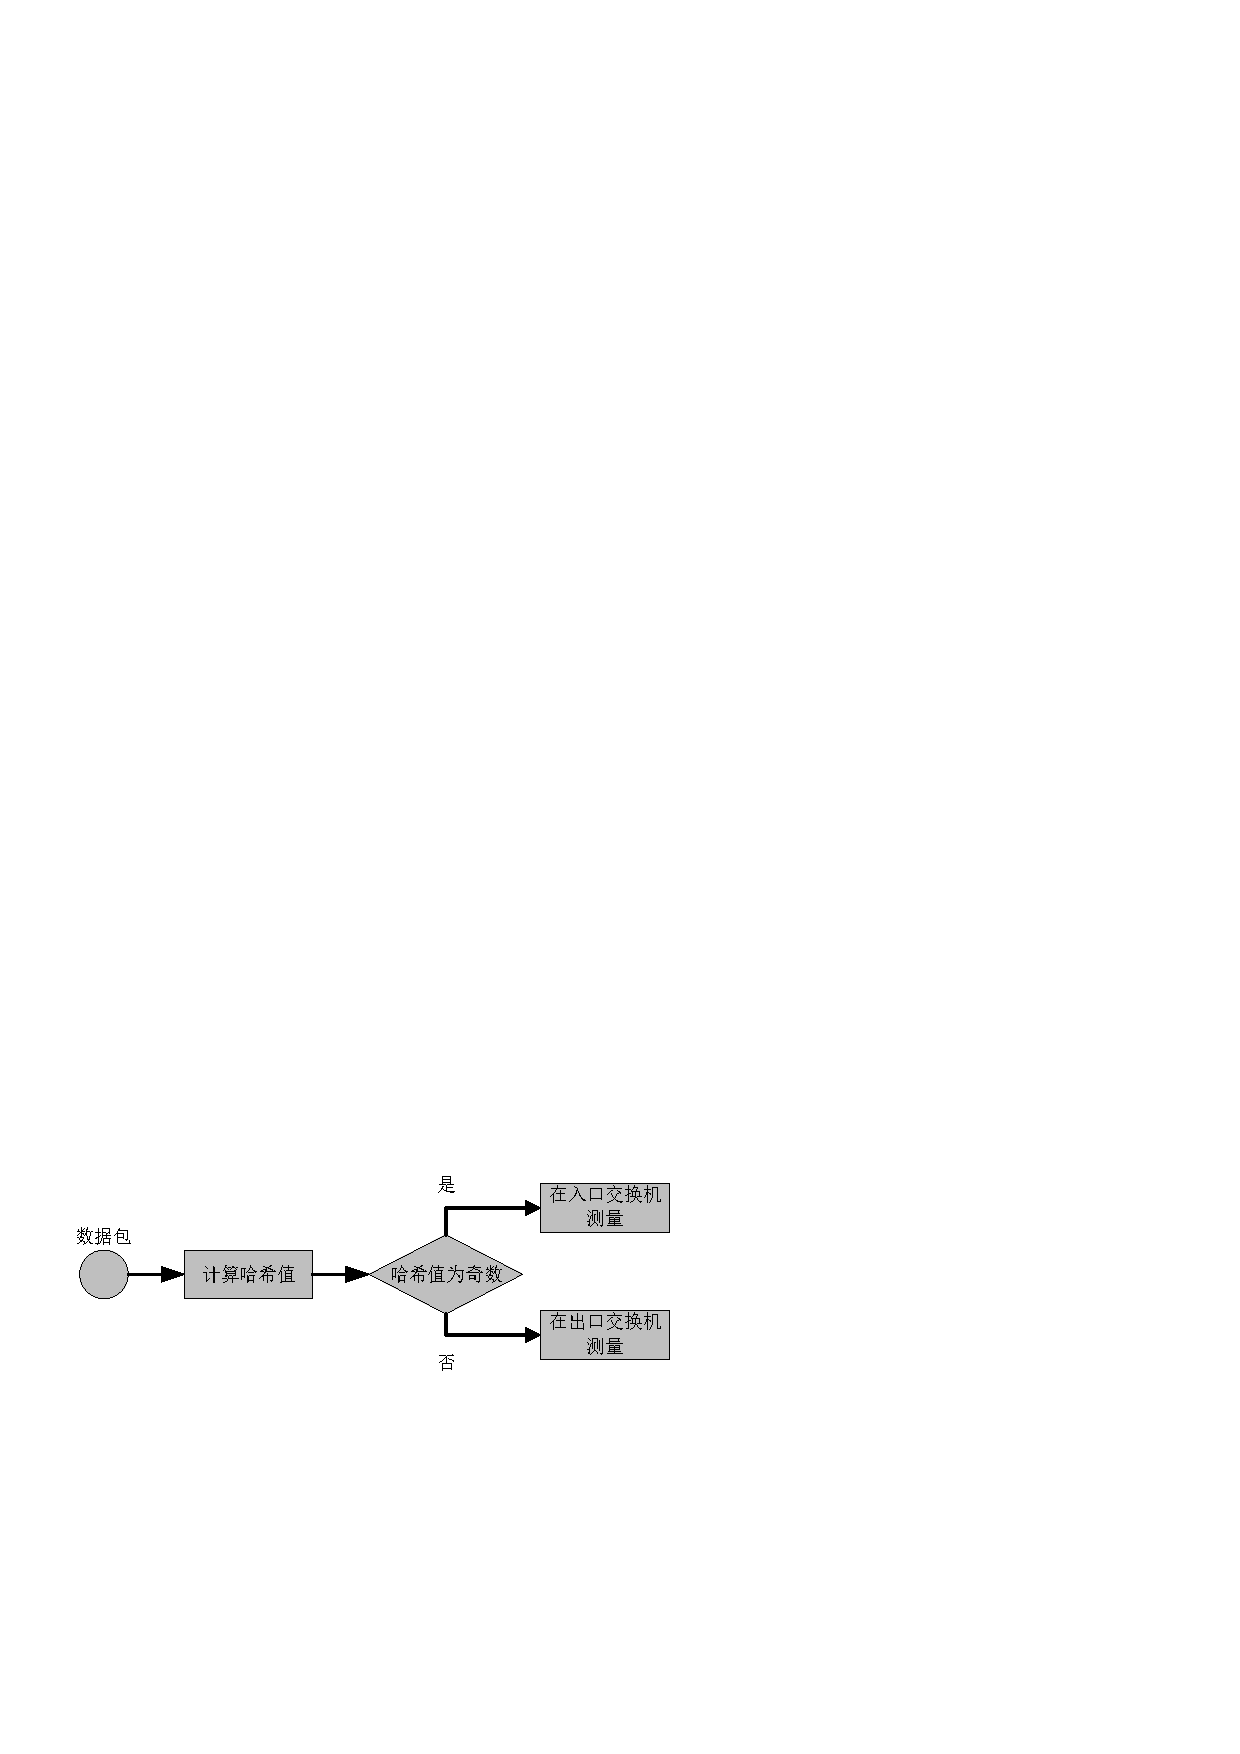
\includegraphics[width=0.7\linewidth]{fig/filter_measure.pdf}
   \caption{协作式CountMax的示意图}
   \label{fig:filtermeasurement}
\end{figure}

另一种降低计算负载的方法是减少CountMax所需要处理的数据包的个数。要测量流的流量,最简单的方案就是在每一个交换机上都部署一个CountMax,并且处理经过交换机的所有数据包。
然而,网络中的很多流是要经过多个交换机的(由于CountMax的主要应用是流的重路由,所以实际上我们只关心那些要经过多个交换机的流),同一条流可能会被多个交换机统计,造成资源的浪费。

因此,本文提出了一种“协作”的方法,使用简单的方式保证一条流只会被一个交换机测量。协作式的流量测量的流程如图\ref{fig:filtermeasurement}所示。
每当一个数据包抵达交换机时,交换机首先用一个哈希函数对流的ID进行哈希。这个哈希函数是所有交换机所共享的。
如果哈希的结果是奇数,那么这条流应当被它的入口交换机,也就是路由上的第一个交换机进行测量。反之则被出口交换机所测量。
交换机可以通过这条流的入端口和出端口来判断自己是不是入口交换机或者出口交换机。
和第\ref{chap:gmsc}章中介绍的分布式部署方式不同,协作式CountMax是完全自组织的,无需控制平面的介入。

接下来分析协作式CountMax的估计误差。不失一般性,我们假设网络中只有两个交换机。网络中的所有流都是先经过交换机1,再经过交换机2的。
假设所有流的总流量是$F$,交换机1处理的流量占比是$\gamma_1 $,那么它处理的总流量就是$F_1 =\gamma_1\cdot F $。
相应的,交换机2处理的流量占比是$\gamma_2 $,总流量是$F_2 =\gamma_2\cdot F $。

首先关注交换机1。令$f$代表网络中所有的流当中的一条$\delta$-heavy hitter流,则$f$的流量大于$\delta \cdot F$。
如果$f$是被交换机1所处理的,那么对于被交换机所处理的流的集合而言,$f$是一个$\delta/\gamma_1$-heavy hitter。
根据定理\ref{tm:query}和定理\ref{tm:acc},有如下不等式成立:

\begin{equation}\label{eq:coop_acc}
\left\{
\begin{aligned}
&Pr[1-\frac{e\cdot \gamma_x}{w\cdot \delta}\le \frac{\hat{a}_i}{a_i} \le 1] \ge 1-e^{-\tilde{d}}\\
&E[\tilde{d}]\ge d\cdot(1-\frac{\gamma_x}{w\cdot\delta})
\end{aligned}
\right.
\end{equation}

其中$\gamma_x$ 根据这条流被哪个交换机所测量,而代表 $\gamma_1$ 或 $\gamma_2$。如果定义 $\gamma_m = \max \{\gamma_1, \gamma_2\}$,用$\gamma_m$替换$\gamma_x$,即可得到一个下界。
在最好的情况下,$\gamma_1=\gamma_2=1/2$。
在实际情况中,通过选择足够随机的哈希函数,$\gamma_1$ 和 $\gamma_2$通常都会比较接近。
参照等式\eqref{eq:coop_acc}, 协作式CountMax将$\frac{\hat{a}_i}{a_i}$ 和 $E[\tilde{d}]$ 这两个值的界缩紧为原本的 $\gamma_m $倍。

\chapter{仿真模拟与系统测试}
\section{CountMax的系统集成测试}\label{sec:proto}

为了验证CountMax的可行性,我们基于Open vSwitch软交换机开发了一个原型系统,并测试了我们的sketch。

\subsection{测试指标与基准}\label{sec:testbedmetric}
系统测试中我们采用了3种不同的指标。其中之一是最大链路负载率,在第\ref{subsec:metric}小节中已经定义。另外两种如下:
\begin{enumerate}
	\item
    处理一个包所需的平均CPU时钟周期数。
    第\ref{sec:simulation}节中所述的运行时间会被主机上的其他因素,如代码JIT编译、后台进程等所影响,因此我们采用CPU周期来衡量系统测试中的计算负载\cite{huang2017sketchvisor}。
    通过在sketch代码中插入查询CPU计数器的API,我们可以得到处理一个数据包所需的平均CPU时钟周期数。
	\item
    Sketch每秒可处理的数据包数(pps),即吞吐量。我们一次性发送巨大数量的数据包,来测试在占满计算资源的情况下,sketch的处理能力。
\end{enumerate}


\subsection{系统实现与设置}
\begin{figure}[ht]
	\centering
	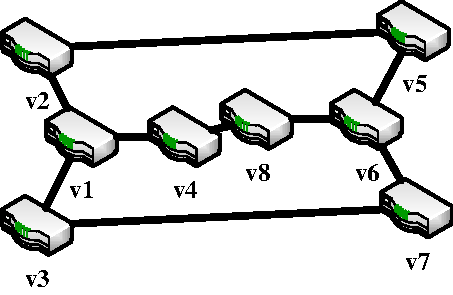
\includegraphics[width=0.68\linewidth]{fig/topo.pdf}
	\caption{\textnormal{系统测试的拓扑。}}
	\label{fig:prototypetopo}
	\note{$v_3,v_4,v_5,v_6$ 分别连接了一个主机。图中未画出控制器和主机。}
\end{figure}

图\ref{fig:prototypetopo}示意了系统测试所用的拓扑。
拓扑中包含一个控制器,6个虚拟交换机,以及4个主机。出于简洁起见,图中没有画出控制器和主机。
控制器使用Ryu \cite{ryu}实现。虚拟交换机基于Open vSwitch (OVS)2.8.2版本\cite{openvswitch}。主机为虚拟主机。
交换机3~6上集成了sketch,并且它们的sketch只处理入站流量。

我们使用C语言实现了CountMax、CountSketch和FSS,使用gcc编译器\cite{gcc}的-O2选项进行优化,并将它们分别集成到OVS的datapath内核模块中。
在OVS处理到达的数据包时,它将会调用sketch来进行更新操作。
sketch监听一个TCP端口用来上报自己的统计数据。

重路由测试的方式与第\ref{sec:simulation}节相似。
在所有的流都处理完毕后,收集sketch的统计数据进行脱机计算。
将计算得出的路由作为流表下发到交换机中,然后再次发送这些流。
通过OVS所搭载的端口统计功能获取链路负载信息。

CPU周期测试的形式为预先生成好大量的伪数据包,将它们的信息直接提供给一个单独的sketch实例,此过程中没有产生实际的网络流量。

CPU周期测试运行在Windows 10操作系统上,其他的测试则运行在Ubuntu 14.04 LTS,Linux内核版本4.10。

集成了CountMax的OVS内核模块的代码公布在https://github.com/VALLIS-NERIA/ovs-datapath。
 
\subsection{测试结果}

\begin{figure}[!t]
	\centering
	\begin{minipage}[t]{0.48\linewidth}		
		%\begin{figure}[!t]
		\centering
		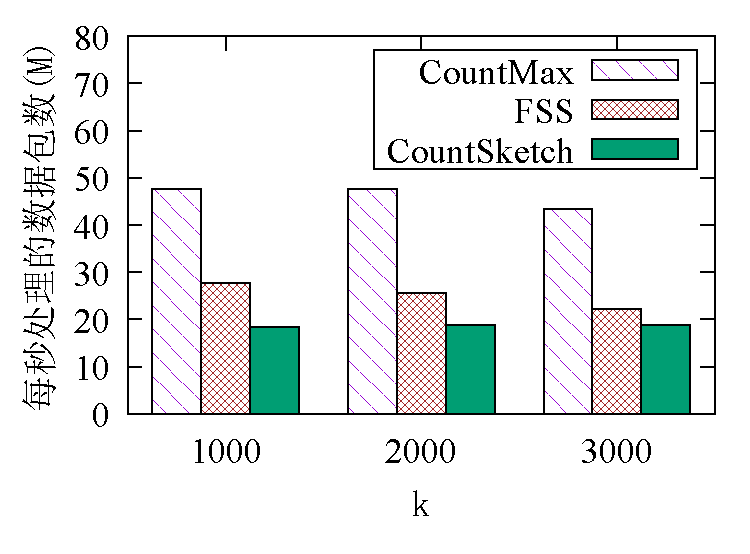
\includegraphics[width=\linewidth]{fig/throughput.pdf}
		\caption{\textnormal{不同sketch的吞吐量随$k$变化。}}
		\label{fig:prototype,bandwidth}
		%\end{figure}
	\end{minipage}\vspace{-0.6em}\hspace{0.4em}
	\begin{minipage}[t]{0.48\linewidth}
	\centering
        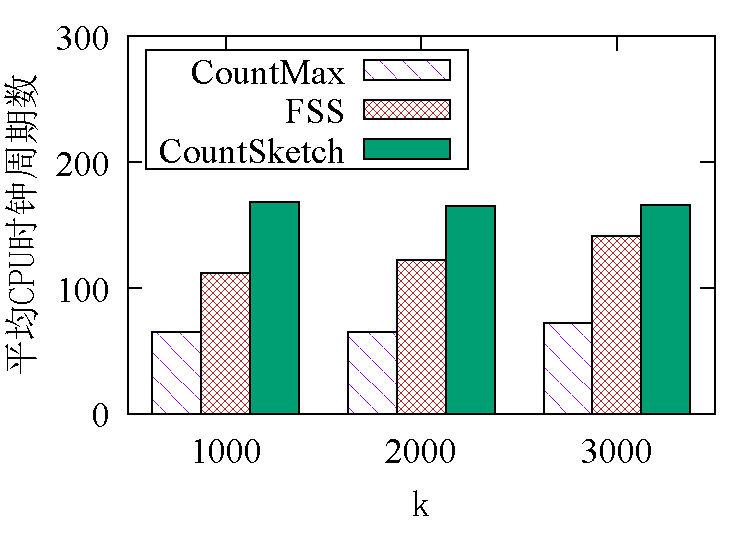
\includegraphics[width=\linewidth]{fig/k_cpu_2000.pdf}
        \caption{\textnormal{处理数据包的平均CPU周期。}}
        \label{fig:prototype,cycle}
	\end{minipage}\vspace{-0.6em}
\end{figure}


\begin{figure}[!t]
	\centering
	\begin{minipage}[t]{0.48\linewidth}		
		%\begin{figure}[!t]
		\centering
		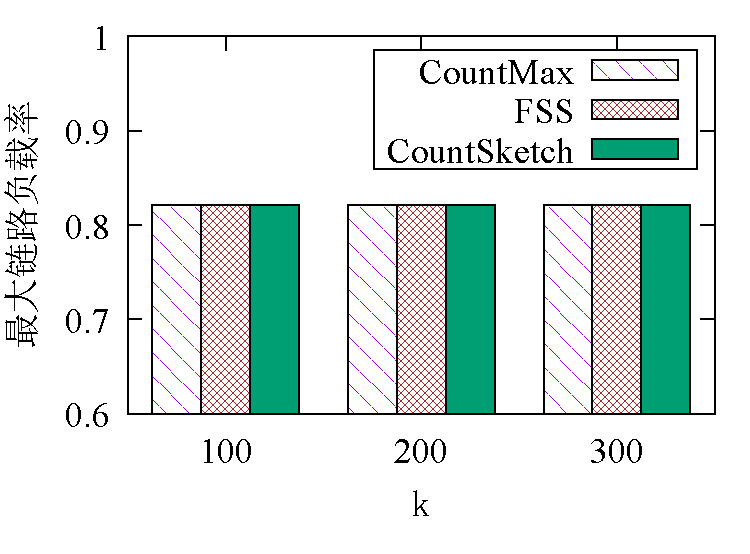
\includegraphics[width=\linewidth]{fig/proto_k_load_2000.pdf}
		\caption{\textnormal{最大链路负载与$k$,2000条流。}}
		\label{fig:prototype,load,k}
		%\end{figure}
	\end{minipage}\vspace{-0.6em}\hspace{0.4em}
	\begin{minipage}[t]{0.48\linewidth}
		\centering
		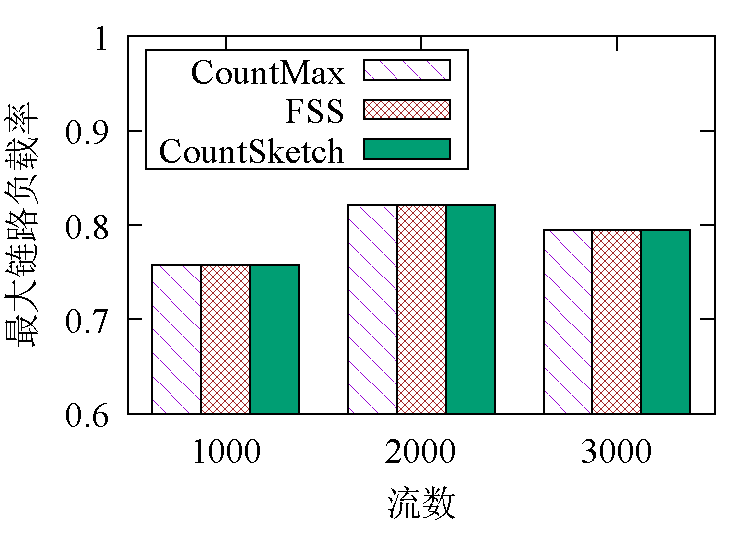
\includegraphics[width=\linewidth]{fig/proto_flow_load_200.pdf}
		\caption{\textnormal{最大链路负载与流数,$k=100$。}}
		\label{fig:prototype,load,flow}
	\end{minipage}\vspace{-0.6em}
\end{figure}


%Figs. \ref{fig:prototype,bandwidth} and \ref{fig:prototype,cycle} are about the computing overhead evaluation.
图\ref{fig:prototype,bandwidth} 体现了不同sketch的吞吐率。
最初我们将sketch装载到一个单独的OVS实例上,并对它进行压力测试,结果发现sketch对于吞吐率的影响不到1\%。
经过深入研究,我们发现OVS作为软交换机,绝大多数的计算资源都被用来和物理网卡进行数据交换以及流表的匹配,sketch占用的计算资源显得微不足道。
而在实体交换机中,流表匹配和包的转发由专用芯片进行处理,sketch的计算负载并不是微不足道的。
因此最终我们将sketch抽离出来,使用生成的数据包单独进行压力测试。
图\ref{fig:prototype,bandwidth}显示,在我们的测试平台下,CountMax、FSS和CountSketch每秒分别可以处理50M、30M和20M个数据包。

在CPU测试当中,每组测试运行了10次以尽可能消除误差。图\ref{fig:prototype,cycle}显示CountMax、FSS、CountSketch处理每个数据包分别需要60、110、170个时钟周期。
代入第\ref{sec:observation}节的假设,计算可得CountMax、FSS、CountSketch将会分别消耗26\%、44\%和68\%的CPU时间。
当网络负载变重,如$\beta=0.6$时,CountMax会消耗约72\%的CPU时间,而FSS和CountSketch则会消耗132\% 和 204\%的CPU时间。
后两者的数字超过了100\%,这意味着统计数据可能会出现丢失的情况,交换机上的其它功能可能无法正常运行。
对于CountMax而言,交换机上的其它功能仍有可能能够正常运行。
与前一节中的图\ref{fig:time,k}相比,这一组测试中CountMax与另两种sketch的计算负载的差距没有那么显著。
其原因在于系统测试使用的是C语言实现,启用了优化,且其中用到的数据结构是专门编写的;
而仿真模拟中使用的是编译成中间代码的C\#语言,没有开启优化,且用到的哈希堆是由系统库中通用的哈希表和小根堆拼凑而成的。
另外,系统测试中的$k$的规模也远小于仿真模拟中的$k$,因而$O(\log{k})$的时间复杂度显示的不明显。

图\ref{fig:prototype,load,k} 和图 \ref{fig:prototype,load,flow}是关于重路由性能的。
从中可以看到$k=100$即可处理2000条流,而随着流数的增加,链路负载也在增加。
总体上结果与第\ref{sec:simulation}节中的结果类似,3种sketch在重路由的方面性能几乎一致。

系统测试的结果显示,CountMax消耗的CPU计算资源分别比FSS和CountSketch少约40\%和60\%,而在应用于重路由方面时,三者的性能几乎完全相同。
因而,CountMax在没有牺牲重路由性能的前提下,降低了处理数据包的计算负载。


\section{小结}
本章首先确定了CountMax的设计目标,随后提出了CountMax的算法,通过数学上的分析证明了CountMax的测量误差的有界性以及CountMax在时间复杂度上的优越性,并介绍了CountMax在重路由中的应用和协作式部署。
其次,通过仿真模拟和系统集成测试,详尽评测了CountMax与CountSketch和FSS之间的性能差异。
测试结果显示,与CountSketch和FSS相比,CountMax能够在几乎没有损失测量精确度的前提下降低约一半的计算负载。